\documentclass[a4paper]{article}

\usepackage[english]{babel}
\usepackage[utf8]{inputenc}
\usepackage{amsmath, amsthm, amssymb}
\usepackage{physics}
\usepackage{graphicx}
\usepackage[colorinlistoftodos]{todonotes}
\usepackage{csquotes}
\usepackage{booktabs}
\usepackage[
    backend=biber,
    style=authoryear,
    natbib=true,
    url=false, 
    doi=false,
    eprint=false
]{biblatex}

\newtheorem{define}{Definition}
\newtheorem{model}{Model}

\newcommand{\prob}[2]{\Pr(#1 \mid #2)}
\newcommand{\set}{\mathrm}
\newcommand{\qset}[2]{\set{#1}/#2}

\addbibresource{../../../../literature/literature.bib}
\graphicspath{{fig/}} % Directory in which figures are stored

\title{Quantifying Differential Methylation in Structured Populations}
\author{\"Onder Kartal}
\date{\today}

\begin{document}

\maketitle

\begin{abstract}

  The mapping and quantification of epigenetic differences between
  cells, tissues, and organisms at genome scale is critical to
  determine effects of environment, differentiation, and reproduction
  on gene function.  The techniques to detect epigenetic signals are
  based on next-generation sequencing.  However, this technology only
  produces a random sample of sequence reads and a crucial part of
  signal detection is done in silico.  In the case of DNA methylation,
  sodium bisulfite treated reads are aligned to the reference genome
  to build genome-scale methylation tables.

  Here, we address the problem of reliably detecting differentially
  methylated cytosines (DMCs) based on methylation tables.  We
  investigate an information-theoretic measure, the Jensen-Shannon
  Divergence (JSD), to scan the genome for DMCs.  JSD is a
  well-founded and very general measure of statistical dependence that
  can be applied to any probabilistic description of the methylation
  state and does not suffer from shortcomings of correlation-based
  measures or standard statistical tests.

  We set up a computational pipeline to calculate JSD along the genome
  for a population.  We extend the definition of JSD to account for
  population structure similar to Sewall Wright's F-statistics.  This
  allows the detection of DMCs between subpopulations, for example
  different lines, demes, or different treatment groups.  The analysis
  of published methylomes of Arabidopsis reveals that population
  diversity is consistently higher for cytosines in a CG context than
  those in a CHG or CHH context.  As CG methylation is enriched in
  gene bodies, especially exons, this suggests differences in gene
  activity.

  In conclusion, we have established that JSD allows the
  straightforward and accurate detection of DMCs while additionally
  quantifying the extent of differentiation.

\end{abstract}

\section{Introduction}
\label{sec:introduction}

% Variation is a crucial concept in biology. Its quantification goes
% back to the research program of the biometricians in the 19th
% century. This line of development is associated with the names of
% Francis Galton and Karl Pearson. In the hands of Ronald Fisher the
% variation of quantitative traits was reconciled with Mendel's
% concept of particulate inheritance~CITE. This was the birth of
% quantitative genetics and, with seminal contributions from Sewall
% Wright and John Haldane, of population genetics. This led to a
% research program that aims at quantifying genetic variation and
% associating this variation with that of phenotypic traits and
% evolutionary concepts like fitness and mutation as well as
% ecological phenomena like geographic distribution. Thus, variation
% in heritable properties lies at the heart of many questions. This
% has not changed in principle with the advent of modern sequencing
% technologies but the resolution we can achieve nowadays allows us to
% address questions at the level of nucleotide diversity.

In recent years it has become increasingly clear that gene function is
not determined by genetic information, that is DNA sequence,
alone. Epigenetics is
\begin{quote}
  the study of mitotically and/or meiotically heritable changes in
  gene function that can not be explained by changes in DNA
  sequence~CITE
\end{quote}
Cytosine (C) Methylation is one of the best-characterized epigenetic
signals. It is associated with gene silencing when found in promoters
and with active transcription when found in gene bodies. It is also an
effective mechanism to silence transposons.

The state-of-the-art method to measure the methylation state accross
the whole genome at single-base-pair resolution is to sequence
bisulfite-treated DNA fragments. This is followed essentially by two
computational steps~CITE: read alignment to the reference genome and
inference of the methylation level at each locus. This analysis
results in a methylation table that allows to retrieve the number of
methylated and unmethylated reads for each covered C.

The possibility to generate methylomes with relative ease has led to
large scale studies that try to investigate the extent of differential
methylation in a population of cells or organisms. By differential
methylation we mean single differentially methylated cytosines (DMCs)
or spatially clustered collections of DMCs, called differentially
methylated regions (DMRs). Typically, the sample population is
structured in the sense that each individual belongs at least to a
certain group. The partitioning can be, for example, in terms of
lineages, generations, demes or experimental treatments.

A basic task is then to quantify the methylation diversity accross the
genome within and between subpopulations. We argue that the most
reasonable way to do so, is to use an information-theoretic measure
based on entropy. Our basic reasoning goes as follows: Our degree of
belief regarding the methylation state at a locus is described by a
probability distribution function (PDF). This representation of our
knowledge accounts as well for the uncertainty in a quantitative
fashion. In this setting, assessing the difference between loci means
measuring the difference between PDFs. Information theory provides the
appropriate measures to quantify the difference between PDFs by
quantifying how much information is shared between the PDFs. This is
the most general measure of statistical dependence we are aware of. In
particular, the Jensen-Shannon divergence is a suitable measure of
differences in a population of PDFs.

\section{Material and Methods}
\label{sec:material-methods}

Our method of inference is based on comparing probabilistic
representations of methylation states. To follow the argument, it is
necessary to understand central concepts from probability theory and
information theory. Here, we want to give a brief overview of these
concepts and their implementation in computer code to scan genomic
regions based on methylome data.

\subsection{Basic Concepts}
\label{sec:basic-concepts}

A probabilistic model requires the definition of a \textbf{sample
  space} $\Omega$. This set contains all possible states of a system
or at least those states that we care to model. If we conduct an
experiment we can predict the outcome only to a certain degree due to
missing information. The uncertainty is either about the laws that
govern the system, about parameter values that are outside of our
control or about all the intricacies of the experiment itself. Another
common source of uncertainty is the deliberate ignorance of processes
that may interfere with the modelled process but whose influence we
are unable to specify. Therefore, we model such an experiment as a
\textbf{random variable} $X$. The name is misleading, since $X$ is
actually a function, $X: \Omega \longmapsto \mathbb{R}$, that maps
each possible state to a real number. Thus, it is customary to also
refer to the value of $X$ as the random variable. We are not keen, at
the moment, to resolve this ambiguity in the literature. In essence,
the value of a random variable is a proxy for a single or several
states of the system and its observation is an \textbf{event}. A
random variable that maps a non-singleton subset of its domain
$\Omega$ to a single value is typically used if we are interested in
an outcome that is compatible with any of the states in the subset. An
event written as $(X=x)$, where $x \in X(\Omega)$, is defined formally
in terms of the sample space as
\begin{equation}
  \label{eq:randevent}
  \left( X=x \right) = \left\{ \omega: X(\omega)=x \right\}.
\end{equation}

A \textbf{probability measure} $\Pr$ is a function that assigns a
number in the range $[0, 1]$ to each event and fulfills the condition
$P(\Omega)=1$. The normalization guarantees that probability is a
conserved quantity that can only be redistributed among the events.
%---http://math.stackexchange.com/a/298992
The notion of a probability measure is closely related to that of a
\textbf{probability distribution}. The distribution function is
central to our approach to detect differences in methylation. In the
discrete case, the probability is concentrated in a countable set of
points and the discrete distribution is called a \textbf{probability
  mass function} (pmf). For $N$ possible outcomes, $X=\{ x_1, x_2,
\ldots, x_N \}$, the probabilities of the events are given by
$\Pr(X=x_1)$, $\Pr(X=x_2)$, etc., and the normalization condition
reads $\sum_k \Pr(X=x_k) = 1$. We will denote the pmf as $p(x_k)$
instead of the more verbose $\Pr(X=x_k)$. If the random variable is
continuous, an event is represented by an interval $(a < X < b)$ whose
probability is
\begin{equation}
\Pr(a < X < b) = \int_a^b p(x)\,dx.
\end{equation}
The normalization condition reads $\Pr(\Omega)=\int_{X(\Omega)}
p(x)\,dx = 1$, where $p(x)$ is the \textbf{probability density
  function} (pdf). In contrast to the pmf, note that $p(x) \neq
\Pr(X=x)$.

If we consider more than one random variable or a single event we are
concerned with questions like: How likely is it that distinct events
will co-occur? Does the probability of an event change if we have
information that another event applies? What does it mean that two
events are independent? To answer these questions we have to introduce
the important concept of \textbf{conditional probability}. When we
write $\Pr(A)$ for the probability of any event we actually mean
$\prob{A}{I}$, where the notation `$\mid$' means `conditional on' or
`given that'. The symbol $I$ summarizes all background information
that is implied when we speak about probabilities of $A$. Especially
in the Bayesian camp, conditional probabilities are often taken as the
primitive notions of probability theory~\citep{jaynes2003,sivia2006}.
According to this viewpoint, there is no such thing as an
unconditional probability. Based on this qualification, the product
rule explains how \textbf{joint probabilities} are composed. For two
events $A$ and $B$ we have
\begin{align}
\label{eq:product}
\begin{split}
\prob{AB}{I} &= \prob{A}{BI} \times \prob{B}{I} \\
&= \prob{B}{AI} \times \prob{A}{I},
\end{split}
\end{align}
The conditional probabilities on the right-hand side highlight the
fact that the events may be dependent. If the two events are
independent then conditioning on one event does not confer any
information about the other event and we can write
$\prob{A}{BI} = \prob{A}{I}$ (analogous for $\prob{B}{AI}$). This
leads to the familiar equation for \textbf{statistical independence},
\begin{equation}
\label{eq:independence}
\prob{AB}{I} = \prob{A}{I} \times \prob{B}{I}.
\end{equation}
The existence of joint probabilities carries over to distribution
functions, of course. For two random variables $X$ and $Y$ we will
write the joint distributions as $p(x_k, y_k)$ for the pmf and as
$p(x,y)$ for the pdf.

% Note, that by and large we follow the classic terminology as put
% forward by Kolmogorov. However, we would like to point out that on a
% technical level this is compatible with the viewpoint of probability
% as inductive logic~\citep{jaynes2003} and thus we do not require
% that probability measures can be assigned to presumably random
% events only. Any system about which we have incomplete information
% but want to make quantitative statements is a candidate for
% probabilistic modeling.

Two central notions of this paper are Shannon Entropy and
Jensen-Shannon Divergence. Claude Shannon noticed that a quantity he
called entropy (now commonly referred to as information or Shannon
entropy) can be used to define information rigorously and to develop a
mathematical theory of communication~\citep{shannon1948}.
\begin{define}[Shannon Entropy]
\label{def:shannon}
Given a discrete PDF $f$ the Shannon entropy $H$ quantifies the
average degree of uncertainty in predicting any elementary event
$x_k \in X$:
\begin{equation}
\label{eq:entropy}
H(f) = \sum_k p(x_k) \log_2 \frac{1}{p(x_k)}~~\text{\emph{(in $bits$).}}
\end{equation}
\end{define}

The Jensen-Shannon divergence was explicitly introduced as a
divergence measure to quantify the similarity of PDFs
by~\citet{lin1991}.
\begin{define}[Jensen-Shannon Divergence]
\label{def:jsd}
For a set of distributions $\{f\} = \{f_1, f_2,\ldots\}$ defined over the same sample space $X$ and weighted by factors $\pi_i \geq 0$ with $\sum_i\pi_i = 1$ the Jensen-Shannon divergence is
\begin{equation}
\label{eq:jsd}
D_\text{JS}(\{f\}) = H\left(\sum_i \pi_i f_i\right) - 
       \sum_i \pi_i H\left(f_i\right),~~\text{\emph{(in $bits$).}}
\end{equation}
\end{define}
Note, that on the left hand side of Eq.~\ref{eq:jsd} we have the
entropy of the finite mixture of the input distributions,
$H(f_\text{mix})$, from which the (weighted) average entropy
$\overline{H}$ of the distributions is subtracted.
Figure~\ref{fig:jsd_explain} illustrates that this difference is
always non-negative and thus mixing of distributions can only lead to
an increase in entropy, hence uncertainty. In short, JSD quantifies
the difference between distributions by quantifying the information
loss due to mixing.

% search for `kullback leibler divergence continuous` on google or
% additionally for estimation, this shows papers/videos e.g. of
% perez-cruz and others which shows that the KLD-based formula of JSD
% is applicable to densities!
This is also evident by rewriting $D_\text{JS}$ in terms of
Kullback-Leibler Divergence (KLD), $D_\text{KL}$,
\begin{equation}
\label{eq:jsd_kld}
D_\text{JS} = \sum_i \pi_i D_\text{KL}(f_i || f_\text{mix}).
\end{equation}
The KLD $D_\text{KL}(S || T)$ is a directed (non-symmetric) measure of
information loss when approximating a given source distribution $S$ by
a target distribution $T$~\cite{kullback1951}. By using the mixture as
the target distribution and averaging over the distances, JSD becomes
a smoothed and symmetric version of KLD. We will discuss how JSD is
also a measure of statistical dependence and its close relation with
both mutual information and Fisher's information metric.

Diversity vs. diversity indices...

\begin{figure}[hbt!]
  
\centering
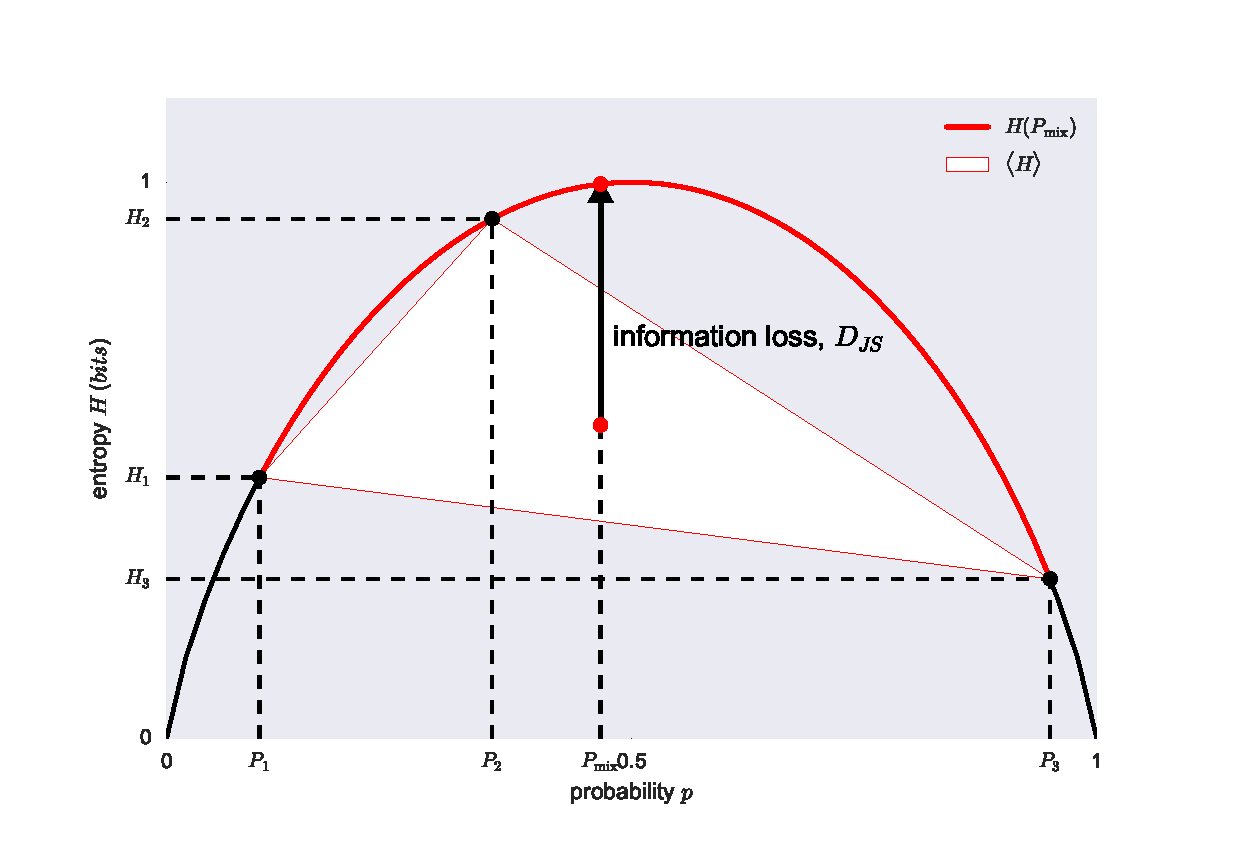
\includegraphics[width=1\textwidth]{jsd_entropy.eps}
\caption{
    Jensen-Shannon Divergence as mixing entropy.
    The graph shows the entropy $H$ of a discrete binary probability distribution function (PDF) $f(\{x_1, x_2\})$ as a function of the probability $p=f(x_1)=1-f(x_2)$.
    The black points show the location of three example PDFs, $f_1$, $f_2$ and $f_3$, in this space.
    Features highlighted in red are quantities entering the Jensen-Shannon Divergence (JSD).
    The entropy of the mixture $H(f_\text{mix})$ can lie anywhere on the red segment of the curve.
    The average entropy, $\langle H \rangle$, is restricted to the area designated by the triangle.
    }
\label{fig:jsd_entropy}


\end{figure}

\subsection{Implementation}
\label{sec:implementation}

\subsection{Data Sources}
\label{sec:data-sources}

\section{Results and Discussion}
\label{sec:results-discussion}

\subsection{Jensen-Shannon Divergence in Structured Populations}
\label{sec:jsd-structured}

It is often necessary or desirable to quantify differences between
populations since most natural and experimental populations are
structured (or subdivided) inherently due to genetic sampling or can
be subdivided into groups that arise by design of the experiment. The
subdivision into groups can be performed at different levels if
hierarchies are present in the population, see
Fig.~\ref{fig:pop-structure}. At any level, it becomes necessary to
consider within-group divergences in order to derive between-group
divergences. As it stands, the expression for JSD gives the
within-group divergence only. This partitioning of divergence is in
principle reminiscent of the partitioning of variance in ANOVA to
calculate differences between two groups.

\todo[inline, color=green!40]{Illustration of Population structure.}

The notion of population structure can be made precise in terms of
equivalence relations. An equivalence relation $R$ over a set
$\set{T}$ (the population) induces a partition of the set into subsets
called equivalence classes (usually referred to as subgroups). Any two
members of the same equivalence class, $a$ and $b$, are said to be
$R$-equivalent or equivalent by $R$, written as $a \sim_R b$. The set
of all equivalence classes is called the quotient set of $\set{T}$ by
$R$, denoted by $\qset{T}{R}$. Of course, different equivalence
relations can be defined on one and the same set, which would lead to
different partitions. In particular, two different equivalence
relations, say $Q$ and $R$, can induce partitions at different levels
in the sense that $a \sim_Q b$ implies $a \sim_R b$. $Q$ is then said
to be a finer relation than $R$ and the $Q$-equivalence class of a
member $a$ is a subset of its $R$-equivalence class.

We give an example that is relevant for populations of Arabidopsis
accessions. The relation $K$=continent would lead to the quotient set
$\qset{T}{K}$ that contains equivalence classes combining samples
originating from the same continent. The relation $L$=country is a
finer relation than $K$ that leads to equivalence classes by countries
in $\qset{T}{L}$. Obviously, for any given member $a$, its
$L$-equivalence class is a subset of its $K$-equivalence class, since
accessions from the same country are also from the same continent of
origin.

Using the concept and terminology of equivalence relations, the
between-group divergence in a set $T$ partitioned by $R$ is actually
the divergence of the quotient set, $J(\qset{T}{R})$. We want to show
how to compute this quantity and how it is related to the total
divergence $J(\set{T})$ and the within-group divergences $J(\set{S})$,
$\set{S} \in \qset{T}{R}$,
\begin{align}
  J(\set{T}) &= H(\pi_i^\set{T}p^i) - \pi_i^\set{T} H(p^i) \qq{and} \\
  J(\set{S}) &= H(\pi_i^\set{S}p^i) - \pi_i^\set{S} H(p^i).
\end{align}
The individual weight vectors $\pi^\set{S}$ and $\pi^\set{T}$ have the
same size but for any subset $\set{S}$ we have $\sum_j \pi^\set{S}_j[j
\in \set{S}] = 1$ and $\pi^\set{S}_i = 0$ for $i \notin \set{S}$. Due
to the convexity of entropy, the average divergence over the quotient
set can never exceed the total divergence,
\begin{equation}
  \label{eq:jsd-avg}
  J(T) \geq \overline{J(\set{S})} \qq{with} \overline{J(\set{S})} = \sum_s\pi^\set{T}_s J(s) [s\in\qset{T}{R}],
\end{equation}
where the weights $\pi_s^\set{T}$ now refer to subsets rather than
individual members of $T$.  It turns out that the mismatch between
total and average divergence is precisely due to the divergence
\emph{between} the subgroups, $J(\qset{T}{R})$:
\begin{align}
  J(\qset{T}{R}) &= J(T) - \overline{J(\set{S})} \\
  % &= H(q^\set{T}) - \sum_i \pi^T_i H(p_i) [i \in T] \\
  % &- \sum_\set{S} \pi^{\qset{T}{R}}_\set{S} \left( H(q^\set{S}) - \sum_i \pi^\set{S}_i H(p_i) [i \in S] \right) [\set{S} \in \qset{T}{R}]\\
  % &= H(q^\set{T}) - \sum_i \pi^T_i H(p_i) [i \in T] \\
  % &- \sum_\set{S} \pi^{\qset{T}{R}}_\set{S} H(q^\set{S})[\set{S} \in \qset{T}{R}]\\
  % &+ \sum_{\set{S},i} \pi^{\qset{T}{R}}_\set{S} \pi^\set{S}_i H(p_i) [i \in S] [\set{S} \in \qset{T}{R}]\\
  &= H(\pi_i^\set{T}p^i) - \pi^\set{T}_s H(\pi_i^s p^i),
\end{align}
which follows from the identity $\pi_i^\set{T} = \pi_\set{S}^\set{T}
\pi^\set{S}_i$ for any given set $\set{S}$ and the canceling of the
term $\pi_i^\set{T} H(p^i)$.

\todo[inline, color=green!40]{Discuss the results, relation to Fst, alpha/beta/gamma Entropy, anova.}

Sewall Wright used the generic notation $ST$ for between-group
correlation in his $F$-statistics \cite{wright1949}. We believe that
using the notation of equivalence relations is more precise and
especially more explicit since it is immediately clear by which
relation the reference set is partitioned.


\subsection{Differentially Methylated Positions}
\label{sec:dmp}

In this section we demonstrate that JSD allows to scan the genome of a
species for differentially methylated positions (DMPs) in an
arbitrarily subdivided population. For this we assume that a
statistical sample of $n$ individuals has been taken from a
population. We further assume that the methylation state at each
cytosine position for each individual is described in terms of a PDF.
Population subdivision refers to a classification of the individuals
into (possibly nested) groups that share some common property or
history. For example, a subgroup may consist of plants that come from
the same habitat or just shared the same experimental treatment. In
cell populations, individuals coming from the same tissue may form a
group that is nested within a group at the level of organs.

To compare cytosine bases across a population sample using PDFs, a
hypothesis space needs to be defined. The choice of a hypothesis space
is not a trivial task -- it already implies a model of the system and
the data-generating process.

\subsubsection{DMPs from discrete representations of methylation state}
\label{sec:dmp-discrete}

\begin{model}[Bernoulli Distribution]\label{mod:bernoulli}
  We assume two mutually exclusive propositions or hypotheses for an
  arbitrary but fixed locus:
\begin{enumerate}
\item $m \equiv$ The locus is methylated.
\item $\neg m \equiv$ The locus is \emph{not} methylated.
\end{enumerate}
In this case the PDF $p(M|I)$ over the set $M=\{m, \neg m\}$ is given
by the probabilities
\begin{align}
p &= \Pr(m|I),\\
q &= \Pr(\neg m|I) = 1 - p.
\end{align}
\end{model}
The Bernoulli distribution is one possible model if we assume that the
locus is either completely methylated or completely unmethylated. This
condition is fulfilled for haploid cells with completely operative
maintenance methylation or, to a certain extent, for cytosine bases in
CG context for plants. It is not an appropriate model if
allele-specific methylation or hemimethylation is possible.

If the background information $I$ does not favor any of the two
propositions, for example, we would encode our indifference by
assigning the prior probabilities
\begin{equation}
p = q = \frac{1}{2}.
\end{equation}
Similar to the case of a fair (i.e. unbiased) coin, this is a
reasonable assignment if we are completely uncertain as to the
methylation state of the locus. To perform the genomic scan, however,
we are interested in the post-data PDFs, $p(M|I,D)$, where the data
consists of bases that map to the locus in question. For that we
interpret the whole sample of bases that map to the locus, with $k$
methylated Cs out of $N$ total reads, as a single Bernoulli trial. In
that case, the posterior probability of methylation is equal to the
sample mean
\begin{equation}
\Pr(m|I,D) = \frac{k}{N}.
\end{equation} 
That is, under the assumption of a Bernoulli likelihood function, we
can use the frequency distribution as the probability distribution.
This is a very crude estimate of the methylation probability without
taking into account sampling bias that is especially problematic for
low sample sizes. Random reads from a DNA library show uneven
distribution or even gaps when mapped to the reference genome.
% In the case of gaps, i.e. no data, the prior PDF is all that we have
% and if our prior is the same for each individual at a particular
% locus there will be no diversity ($J=0$). When we have data, we need
% to use an appropriate likelihood function to do the inference, that
% is we need to define $\Pr(D|m,I)$.
However, frequency distributions are reasonable first approximations
and have been successfully used previously in comparing sequences with
JSD by \cite{grosse2002}. In fact, they have shown that a natural
choice of the weights that enter Eq.~\ref{eq:jsd} allow to mitigate
the effect of sampling bias when comparing PDFs. Using simulations,
they have shown, that sampling bias can be taken into account by using
\begin{equation}
\pi_{i} = \frac{N_{i}}{\sum_i N_{i}}.
\end{equation}

\subsubsection{DMPs from continuous representations of methylation state}
\label{sec:dmp-continuous}

Rather than taking the whole sample of reads as a Bernoulli trial as
in \ref{mod:bernoulli} each single mapped base can be seen as a
Bernoulli trial. This leads naturally to a binomial distribution.
\begin{model}[Binomial Distribution]\label{mod:binomial}
We assume that the methylation bias lies between 0 and 1...
\end{model}
The convenient choice in this case for the prior is that of beta
distribution. In that case one speaks of a conjugate prior since the
posterior PDF is also a beta distribution. It can be shown that the
sample mean is the mode of the posterior PDF if we choose a binomial
likelihood function with a flat prior. However, the posterior PDF now
conveys additional information about the uncertainty of our estimate.
In formulating our problem in a more sensible way we did not throw
away the information that is contained in the sample size...

\subsubsection{Discussion}
\label{sec:dmp-discussion}

\subsection{Differentially Methylated Regions}
\label{sec:dmr}

\subsubsection{JSD in annotated regions}
\label{sec:dmr-annotated}

\subsubsection{JSD-based methylome segmentation}
\label{sec:dmr-segmentation}

\subsubsection{Discussion}
\label{sec:dmr-discussion}

\section{Conclusions}
\label{sec:conclusions}

\printbibliography

\end{document}
